We have split our firmware into a number of separate modules, as shown in figure
\ref{fig:fw_block_diag}. All of the drivers for microcontroller peripherals
such as serial interfaces and the ADC are provided by the nRF52 SDK's hardware
abstraction layer. We are also using some higher level components from the
nRF52 SDK such as the USB CDC-ACM stack, a FAT32 filesystem driver and Nordic's
soft device 140 which is a Bluetooth LE peripheral stack.

These third party components will be used by the software we are planing to
write ourselves which includes the drivers for all of our sensors (IMU, optical
heart rate sensor, air quality sensor and UV light sensor) as well as the signal
processing code required to derive a heart rate from the raw data we receive
from our optical heart rate sensor. While we plan to use a third party file
system implementation we will still need to write the code that allows blocks
to be written to and read from an SD card over an SPI interface.

At the application layer we have three modules. Our data logging service will be
responsible for most of the operation of our device and will continually collect
and log sensor data. The Bluetooth data transfer service will facilitate
accessing the logged data over a Bluetooth interface. Our debugging interface is
intended to expose our firmware functionality over a USB serial interface so
that integration tests can be run on the microcontroller.

\begin{figure}[!htb]
\centering
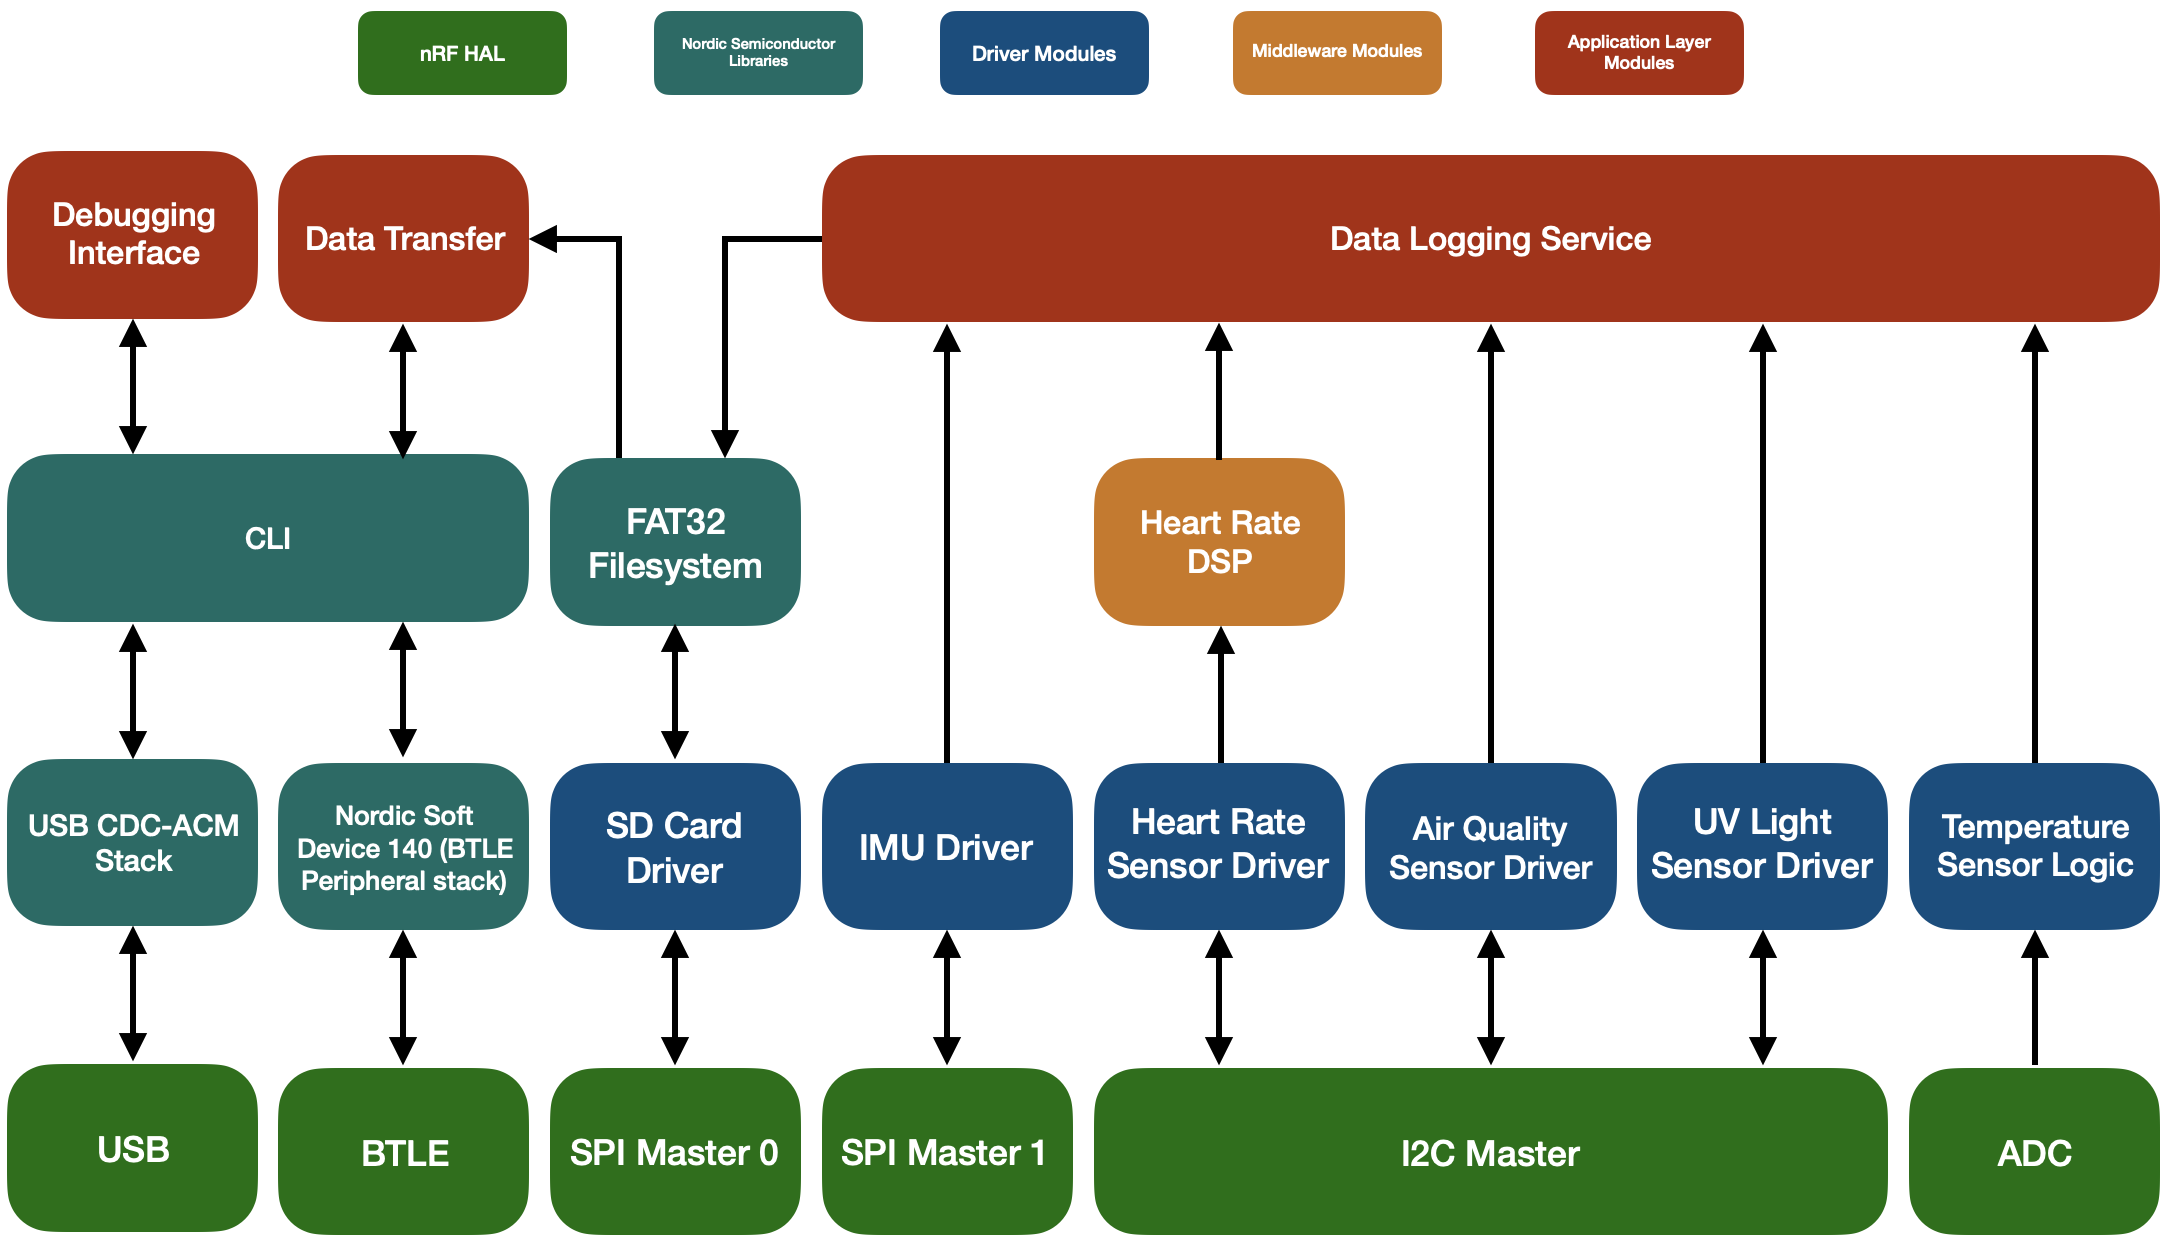
\includegraphics[width=\textwidth]{images/fw_block_diag.png}
\caption{Firmware block diagram.}
\label{fig:fw_block_diag}
\end{figure}

When discussing options on operating systems to use we came to the conclusion 
that most of the benefits of using a RTOS are unnecessary for our application.
Because most of the sensors have internal buffers we can periodically poll
for data without needing formal scheduling pattern.  Other features of 
operating systems such as memory management or preemption would not be
necessary as the services to handle reading data from the sensors and logging
to the SD card using co-operative multi-tasking will be good enough and require
less effort and less ways to go wrong compared to using an RTOS.

The software was written on the bare metal and follows a structure where there
is a central loop which calls services for all components.  Each sensor as well
as the data logging component are implemented as a separate component
to be updated periodically. The drivers read and process the data from the
sensors and write it to a buffer to be written to the SD card. The logging service
maintains a few of these buffers and ensures they get written to the SD card
at reasonable intervals.